\documentclass[aspectratio=169]{beamer}
\usetheme{Madrid}
\usecolortheme{default}

% Packages
\usepackage{graphicx}
\usepackage{amsmath}
\usepackage{amssymb}
\usepackage{tikz}
\usetikzlibrary{arrows,shapes,positioning,calc}
\usepackage{booktabs}
\usepackage{hyperref}

\graphicspath{{./}}

% Custom colors
\definecolor{primary}{RGB}{10,37,64}
\definecolor{secondary}{RGB}{99,91,255}
\definecolor{accent}{RGB}{0,212,255}
\definecolor{success}{RGB}{50,213,131}
\definecolor{warning}{RGB}{255,193,7}
\definecolor{danger}{RGB}{220,53,69}

\setbeamercolor{structure}{fg=secondary}
\setbeamercolor{palette primary}{bg=primary,fg=white}
\setbeamercolor{palette secondary}{bg=secondary,fg=white}
\setbeamercolor{palette tertiary}{bg=accent,fg=white}

% Title page
\title[SE446 - Week 2A]{Introduction to Big Data}
\subtitle{The 5 V's and Why It Matters}
\author{Professor Anis Koubaa}
\institute{
    SE 446\\
    Alfaisal University\\[0.3em]
    \url{https://github.com/aniskoubaa/big_data_course}
}
\date{Spring 2026}
\titlegraphic{\includegraphics[width=1.5cm]{logo.png}}

\begin{document}

% Title slide
\begin{frame}
\titlepage
\end{frame}

% Outline
\begin{frame}{Outline}
\tableofcontents
\end{frame}

% ===== SECTION 1: What is Big Data? =====
\section{What is Big Data?}

\begin{frame}{Motivating Question}
\begin{center}
\Large \textbf{How much data is generated every minute?}
\end{center}

\vspace{1em}

\begin{columns}[T]
\begin{column}{0.48\textwidth}
\textbf{Every 60 seconds:}
\begin{itemize}
    \item 500 hours of YouTube video uploaded
    \item 6 million Google searches
    \item 500,000 tweets posted
    \item 200 million emails sent
\end{itemize}
\end{column}

\begin{column}{0.48\textwidth}
\textbf{The Challenge:}
\begin{itemize}
    \item Too \alert{large} for one machine
    \item Too \alert{fast} for batch processing
    \item Too \alert{complex} for simple queries
    \item Traditional DBs \alert{can't cope}
\end{itemize}
\end{column}
\end{columns}

\vspace{1em}

\begin{alertblock}{Welcome to the Big Data Era}
We need new tools and techniques to handle this scale!
\end{alertblock}
\end{frame}

\begin{frame}{What is Big Data?}
\begin{block}{Definition}
\textbf{Big Data} refers to datasets that are too \textcolor{secondary}{large}, \textcolor{success}{fast}, or \textcolor{warning}{complex} for traditional data processing tools.
\end{block}

\vspace{0.5em}

\begin{itemize}
    \item Cannot fit on a single machine
    \item Cannot be processed in reasonable time
    \item Requires \textbf{distributed computing}
\end{itemize}

\vspace{0.5em}

\begin{alertblock}{Key Insight}
It's not just about \textit{size} — it's about the \textit{challenges} of handling the data.
\end{alertblock}
\end{frame}

\begin{frame}{The Scale of Big Data}
\begin{center}
\begin{tabular}{lll}
\toprule
\textbf{Company} & \textbf{Data Generated} & \textbf{Scale} \\
\midrule
Facebook & 4 PB / day & 250 billion photos \\
YouTube & 500 hours video / minute & 1 billion hours watched/day \\
Twitter & 500 million tweets / day & 6,000 tweets / second \\
Google & 20 PB processed / day & 3.5 billion searches / day \\
\bottomrule
\end{tabular}
\end{center}

\vspace{0.5em}

\begin{block}{Perspective}
1 Petabyte = 1,000 Terabytes = 1,000,000 Gigabytes
\end{block}
\end{frame}

% ===== SECTION 2: The 5 V's =====
\section{The 5 V's of Big Data}

\begin{frame}{The 5 V's of Big Data}
\begin{center}
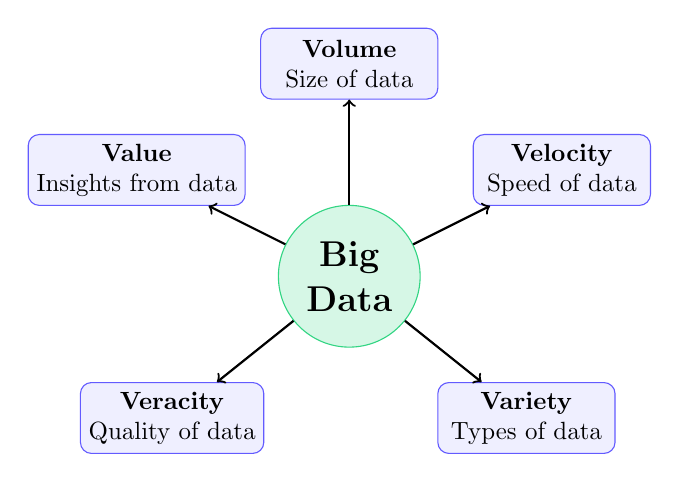
\begin{tikzpicture}[
    box/.style={rectangle, draw=secondary, fill=secondary!10, 
                minimum width=2.5cm, minimum height=1cm, align=center, rounded corners},
    scale=0.9, transform shape
]
    % Center
    \node[circle, draw=success, fill=success!20, 
          minimum size=2cm, align=center, font=\Large\bfseries] (center) {Big\\Data};
    
    % 5 V's
    \node[box] (volume) at (0,3) {\textbf{Volume}\\Size of data};
    \node[box] (velocity) at (3,1.5) {\textbf{Velocity}\\Speed of data};
    \node[box] (variety) at (2.5,-2) {\textbf{Variety}\\Types of data};
    \node[box] (veracity) at (-2.5,-2) {\textbf{Veracity}\\Quality of data};
    \node[box] (value) at (-3,1.5) {\textbf{Value}\\Insights from data};
    
    % Arrows
    \draw[->, thick] (center) -- (volume);
    \draw[->, thick] (center) -- (velocity);
    \draw[->, thick] (center) -- (variety);
    \draw[->, thick] (center) -- (veracity);
    \draw[->, thick] (center) -- (value);
\end{tikzpicture}
\end{center}
\end{frame}

\begin{frame}{Volume: Size of Data}
\begin{columns}[T]
\begin{column}{0.5\textwidth}
\begin{block}{Challenge}
Datasets too large to store or process on a single machine.
\end{block}

\textbf{Examples:}
\begin{itemize}
    \item Genomic data: 100 GB per genome
    \item CERN: 1 PB / month
    \item Autonomous cars: 4 TB / day
\end{itemize}
\end{column}

\begin{column}{0.5\textwidth}
\begin{block}{Solution}
\textbf{Distributed Storage}
\begin{itemize}
    \item HDFS (Hadoop)
    \item Amazon S3
    \item Google Cloud Storage
\end{itemize}
\end{block}
\end{column}
\end{columns}
\end{frame}

\begin{frame}{Velocity: Speed of Data}
\begin{columns}[T]
\begin{column}{0.5\textwidth}
\begin{block}{Challenge}
Data arrives too fast for batch processing.
\end{block}

\textbf{Examples:}
\begin{itemize}
    \item Stock market: millions/second
    \item IoT sensors: continuous stream
    \item Social media: real-time feeds
\end{itemize}
\end{column}

\begin{column}{0.5\textwidth}
\begin{block}{Solution}
\textbf{Stream Processing}
\begin{itemize}
    \item Apache Kafka
    \item Spark Streaming
    \item Apache Flink
\end{itemize}
\end{block}
\end{column}
\end{columns}
\end{frame}

\begin{frame}{Variety: Types of Data}
\begin{center}
\begin{tabular}{lll}
\toprule
\textbf{Type} & \textbf{Description} & \textbf{Examples} \\
\midrule
Structured & Rows \& columns, fixed schema & SQL tables, Excel \\
Semi-structured & Flexible schema, self-describing & JSON, XML, logs \\
Unstructured & No predefined format & Images, videos, emails \\
\bottomrule
\end{tabular}
\end{center}

\vspace{0.5em}

\begin{alertblock}{Key Insight}
80\% of enterprise data is \textbf{unstructured}!
\end{alertblock}
\end{frame}

\begin{frame}{Veracity \& Value}
\begin{columns}[T]
\begin{column}{0.5\textwidth}
\begin{block}{Veracity: Data Quality}
\begin{itemize}
    \item Missing values
    \item Inconsistent formats
    \item Noise and outliers
    \item Fake data (bots, spam)
\end{itemize}

\vspace{0.3em}

\textit{``Garbage in, garbage out''}
\end{block}
\end{column}

\begin{column}{0.5\textwidth}
\begin{block}{Value: Extracting Insights}
\begin{itemize}
    \item Predictive analytics
    \item Customer segmentation
    \item Fraud detection
    \item Recommendation engines
\end{itemize}

\vspace{0.3em}

\textit{``The goal of Big Data''}
\end{block}
\end{column}
\end{columns}
\end{frame}

% ===== SECTION 3: Why Traditional Databases Fail =====
\section{Why Traditional Databases Fail}

\begin{frame}{Limitations of RDBMS}
\begin{center}
\begin{tabular}{lll}
\toprule
\textbf{Challenge} & \textbf{RDBMS} & \textbf{Big Data} \\
\midrule
Scaling & Vertical (bigger server) & Horizontal (add nodes) \\
Schema & Fixed, predefined & Flexible, schema-on-read \\
Data Types & Structured only & All types \\
Cost & Expensive hardware & Commodity hardware \\
Speed & Slow for massive writes & Parallel distributed writes \\
\bottomrule
\end{tabular}
\end{center}

\vspace{0.5em}

\begin{block}{The Solution}
\textbf{Distributed Systems}: Hadoop, Spark, NoSQL databases
\end{block}
\end{frame}

\begin{frame}{Vertical vs. Horizontal Scaling}
\begin{center}
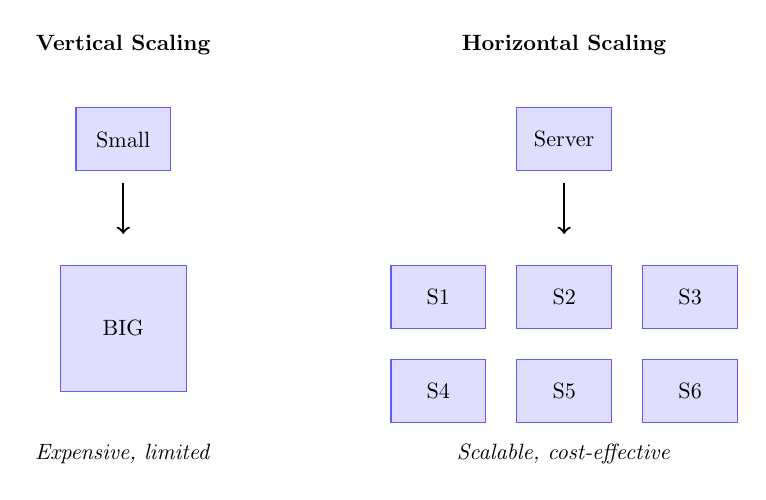
\begin{tikzpicture}[
    server/.style={rectangle, draw=secondary, fill=secondary!20, 
                   minimum width=1.5cm, minimum height=1cm, align=center},
    scale=0.8, transform shape
]
    % Vertical Scaling
    \node at (-4, 3) {\textbf{Vertical Scaling}};
    \node[server, minimum height=1cm] at (-4, 1.5) {Small};
    \draw[->, thick] (-4, 0.8) -- (-4, 0);
    \node[server, minimum height=2cm, minimum width=2cm] at (-4, -1.5) {BIG};
    \node at (-4, -3.5) {\textit{Expensive, limited}};
    
    % Horizontal Scaling
    \node at (3, 3) {\textbf{Horizontal Scaling}};
    \node[server] at (3, 1.5) {Server};
    \draw[->, thick] (3, 0.8) -- (3, 0);
    \node[server] at (1, -1) {S1};
    \node[server] at (3, -1) {S2};
    \node[server] at (5, -1) {S3};
    \node[server] at (1, -2.5) {S4};
    \node[server] at (3, -2.5) {S5};
    \node[server] at (5, -2.5) {S6};
    \node at (3, -3.5) {\textit{Scalable, cost-effective}};
\end{tikzpicture}
\end{center}
\end{frame}

% ===== SECTION 4: The Hadoop Ecosystem =====
\section{The Hadoop Ecosystem}

\begin{frame}{The Hadoop Ecosystem}
\begin{center}
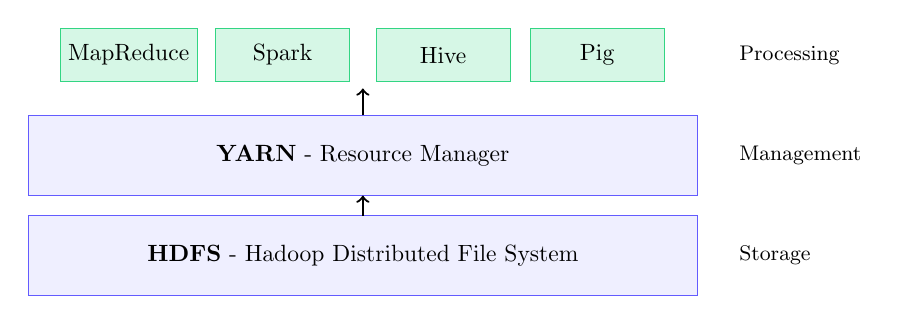
\begin{tikzpicture}[
    layer/.style={rectangle, draw=secondary, fill=secondary!10, 
                  minimum width=10cm, minimum height=1.2cm, align=center},
    app/.style={rectangle, draw=success, fill=success!20, 
                minimum width=2cm, minimum height=0.8cm, align=center},
    scale=0.85, transform shape
]
    % Storage Layer
    \node[layer] (hdfs) at (0, 0) {\textbf{HDFS} - Hadoop Distributed File System};
    
    % Resource Management
    \node[layer] (yarn) at (0, 1.5) {\textbf{YARN} - Resource Manager};
    
    % Processing Layer
    \node[app] at (-3.5, 3) {MapReduce};
    \node[app] at (-1.2, 3) {Spark};
    \node[app] at (1.2, 3) {Hive};
    \node[app] at (3.5, 3) {Pig};
    
    % Labels
    \node[right] at (5.5, 0) {\small Storage};
    \node[right] at (5.5, 1.5) {\small Management};
    \node[right] at (5.5, 3) {\small Processing};
    
    % Arrows
    \draw[->, thick] (0, 0.6) -- (0, 0.9);
    \draw[->, thick] (0, 2.1) -- (0, 2.5);
\end{tikzpicture}
\end{center}

\vspace{0.3em}

\begin{block}{This Course Covers}
HDFS, MapReduce, Hive, Spark, Kafka (Streaming)
\end{block}
\end{frame}

% ===== SECTION 5: Summary =====
\section{Summary}

\begin{frame}{Summary: Key Takeaways}
\begin{enumerate}
    \item \textbf{Big Data} = Volume + Velocity + Variety + Veracity + Value
    \vspace{0.3em}
    \item \textbf{Three data types}: Structured, Semi-structured, Unstructured
    \vspace{0.3em}
    \item \textbf{RDBMS limitations} solved by distributed systems
    \vspace{0.3em}
    \item \textbf{Hadoop Ecosystem}: HDFS (storage), YARN (resources), Spark/Hive (processing)
\end{enumerate}

\vspace{0.5em}

\begin{block}{Next Session}
\textbf{HDFS Architecture}: NameNode, DataNode, Replication
\end{block}
\end{frame}

\begin{frame}{Homework}
\begin{enumerate}
    \item Watch the pre-class video for Session 2B:
    \begin{itemize}
        \item ``HDFS Tutorial'' - Edureka (20 min)
    \end{itemize}
    \vspace{0.3em}
    \item Setup your accounts (if you haven't):
    \begin{itemize}
        \item Google Colab: \url{colab.google.com}
        \item GitHub: \url{github.com}
    \end{itemize}
    \vspace{0.3em}
    \item Review the notebook from today's session
\end{enumerate}
\end{frame}

\begin{frame}{}
\begin{center}
\Huge \textbf{Questions?}

\vspace{1em}

\Large Prof. Anis Koubaa\\
\normalsize akoubaa@alfaisal.edu
\end{center}
\end{frame}

\end{document}
